\chapter{Discussion, Future Work, and Conclusion} \label{conclusion}
\section{Discussion}
Vulture has shown that word-gesture keyboards are beneficial to mid-air text-entry by surpassing earlier work and reaching a text-entry rate of 28.1 WPM. However, these keyboards utilized pinching as a means of word separation \cite{ref_vulture}. This thesis aimed to find alternative solutions to word separation and interaction with mid-air, word-gesture keyboards. To seek improvements superior to pinching, this thesis focused on the 3rd-dimension in addition to implementing a bimodal approach. Inconvenient glove-use was replaced with a natural, barehanded gestural interaction.

This thesis suffered from some of the same issues that were experienced in previous work, such as text-entry rates being much slower for mid-air keyboards than touch-based. One reason for this was that participants were required to recouple the gestures in motor space with those on the display \cite{ref_vulture}. This effect was described in detail for many of the results in Chapter~\ref{results}. Another reason, as seen in Vulture and in other studies \cite{ref_vulture,ref_visual_feedback_focus}, was that participants relied heavily on displayed feedback. This was seen in the small amount of latency introduced by the Leap Motion controller when tracking and displaying hand motions on the screen. Some participants reported having to slow hand movement to ensure a more accurate display representation. If movements were made too quickly, the visual display would lag slightly, causing participants to ``overshoot'' characters. A final similarity to Vulture was that the keyboard alternatives forced explicit delimiting of words, adding to the complexity of text-entry. 

\subsection{Pinching Interaction}
This thesis implemented a pinching method using the Leap Motion controller as a metric for comparison against Vulture's pinching method. This was done to compare the pseudo-implementation of word-gesturing versus Vulture's traditional word-gesture keyboard applied to mid-air. The text-entry rate for pinching with a single session was 11.3 WPM, which was consistent with the mean text-entry rate using Vulture ($M = 11.8$ WPM) for a single session \cite{ref_vulture}. Additionally, pinching was 58\% of the text-entry rate of direct touch input, which was proportional to Vulture at 59\% of the text-entry rate of direct touch input \cite{ref_vulture}. These consistent measures provided a baseline for this thesis's mid-air and bimodal keyboard alternatives.

\subsection{3-dimensional Interaction}
This thesis showed initial text-entry rates for utilizing the 3rd-dimension as a means of word separation at 8.6 WPM for the Static-air approach and 9.6 WPM for the Predictive-air approach. These approaches underperformed because of difficulty in mentally coupling word-gestures in motor space with those displayed on the screen, as well as having extra degrees of freedom in the 3rd-dimension when delimiting words via direct interaction with an invisible plane.

The Predictive-air Keyboard was not significantly worse than the Pinch-air Keyboard and warrants further investigation with a repeated-measures, multiple session study. Both the Static-air and Predictive-air suffered from an issue referred to as ``skimming,'' demonstrated in Figure~\ref{arcing_motion} and Figure~\ref{skimming_problem}. The ``skimming'' issue occurred when the natural arcing of the participant's hand during the gesturing motion caused them to lose the simulated touch. This ``skimming'' occurred both during word-gestures and when removing the hand from the plane after having completed a word-gesture. This was more prevalent if a participant's elbow was rested.

\begin{figure}[!t]
	\centering
	\begin{minipage}[t]{2.5in}
		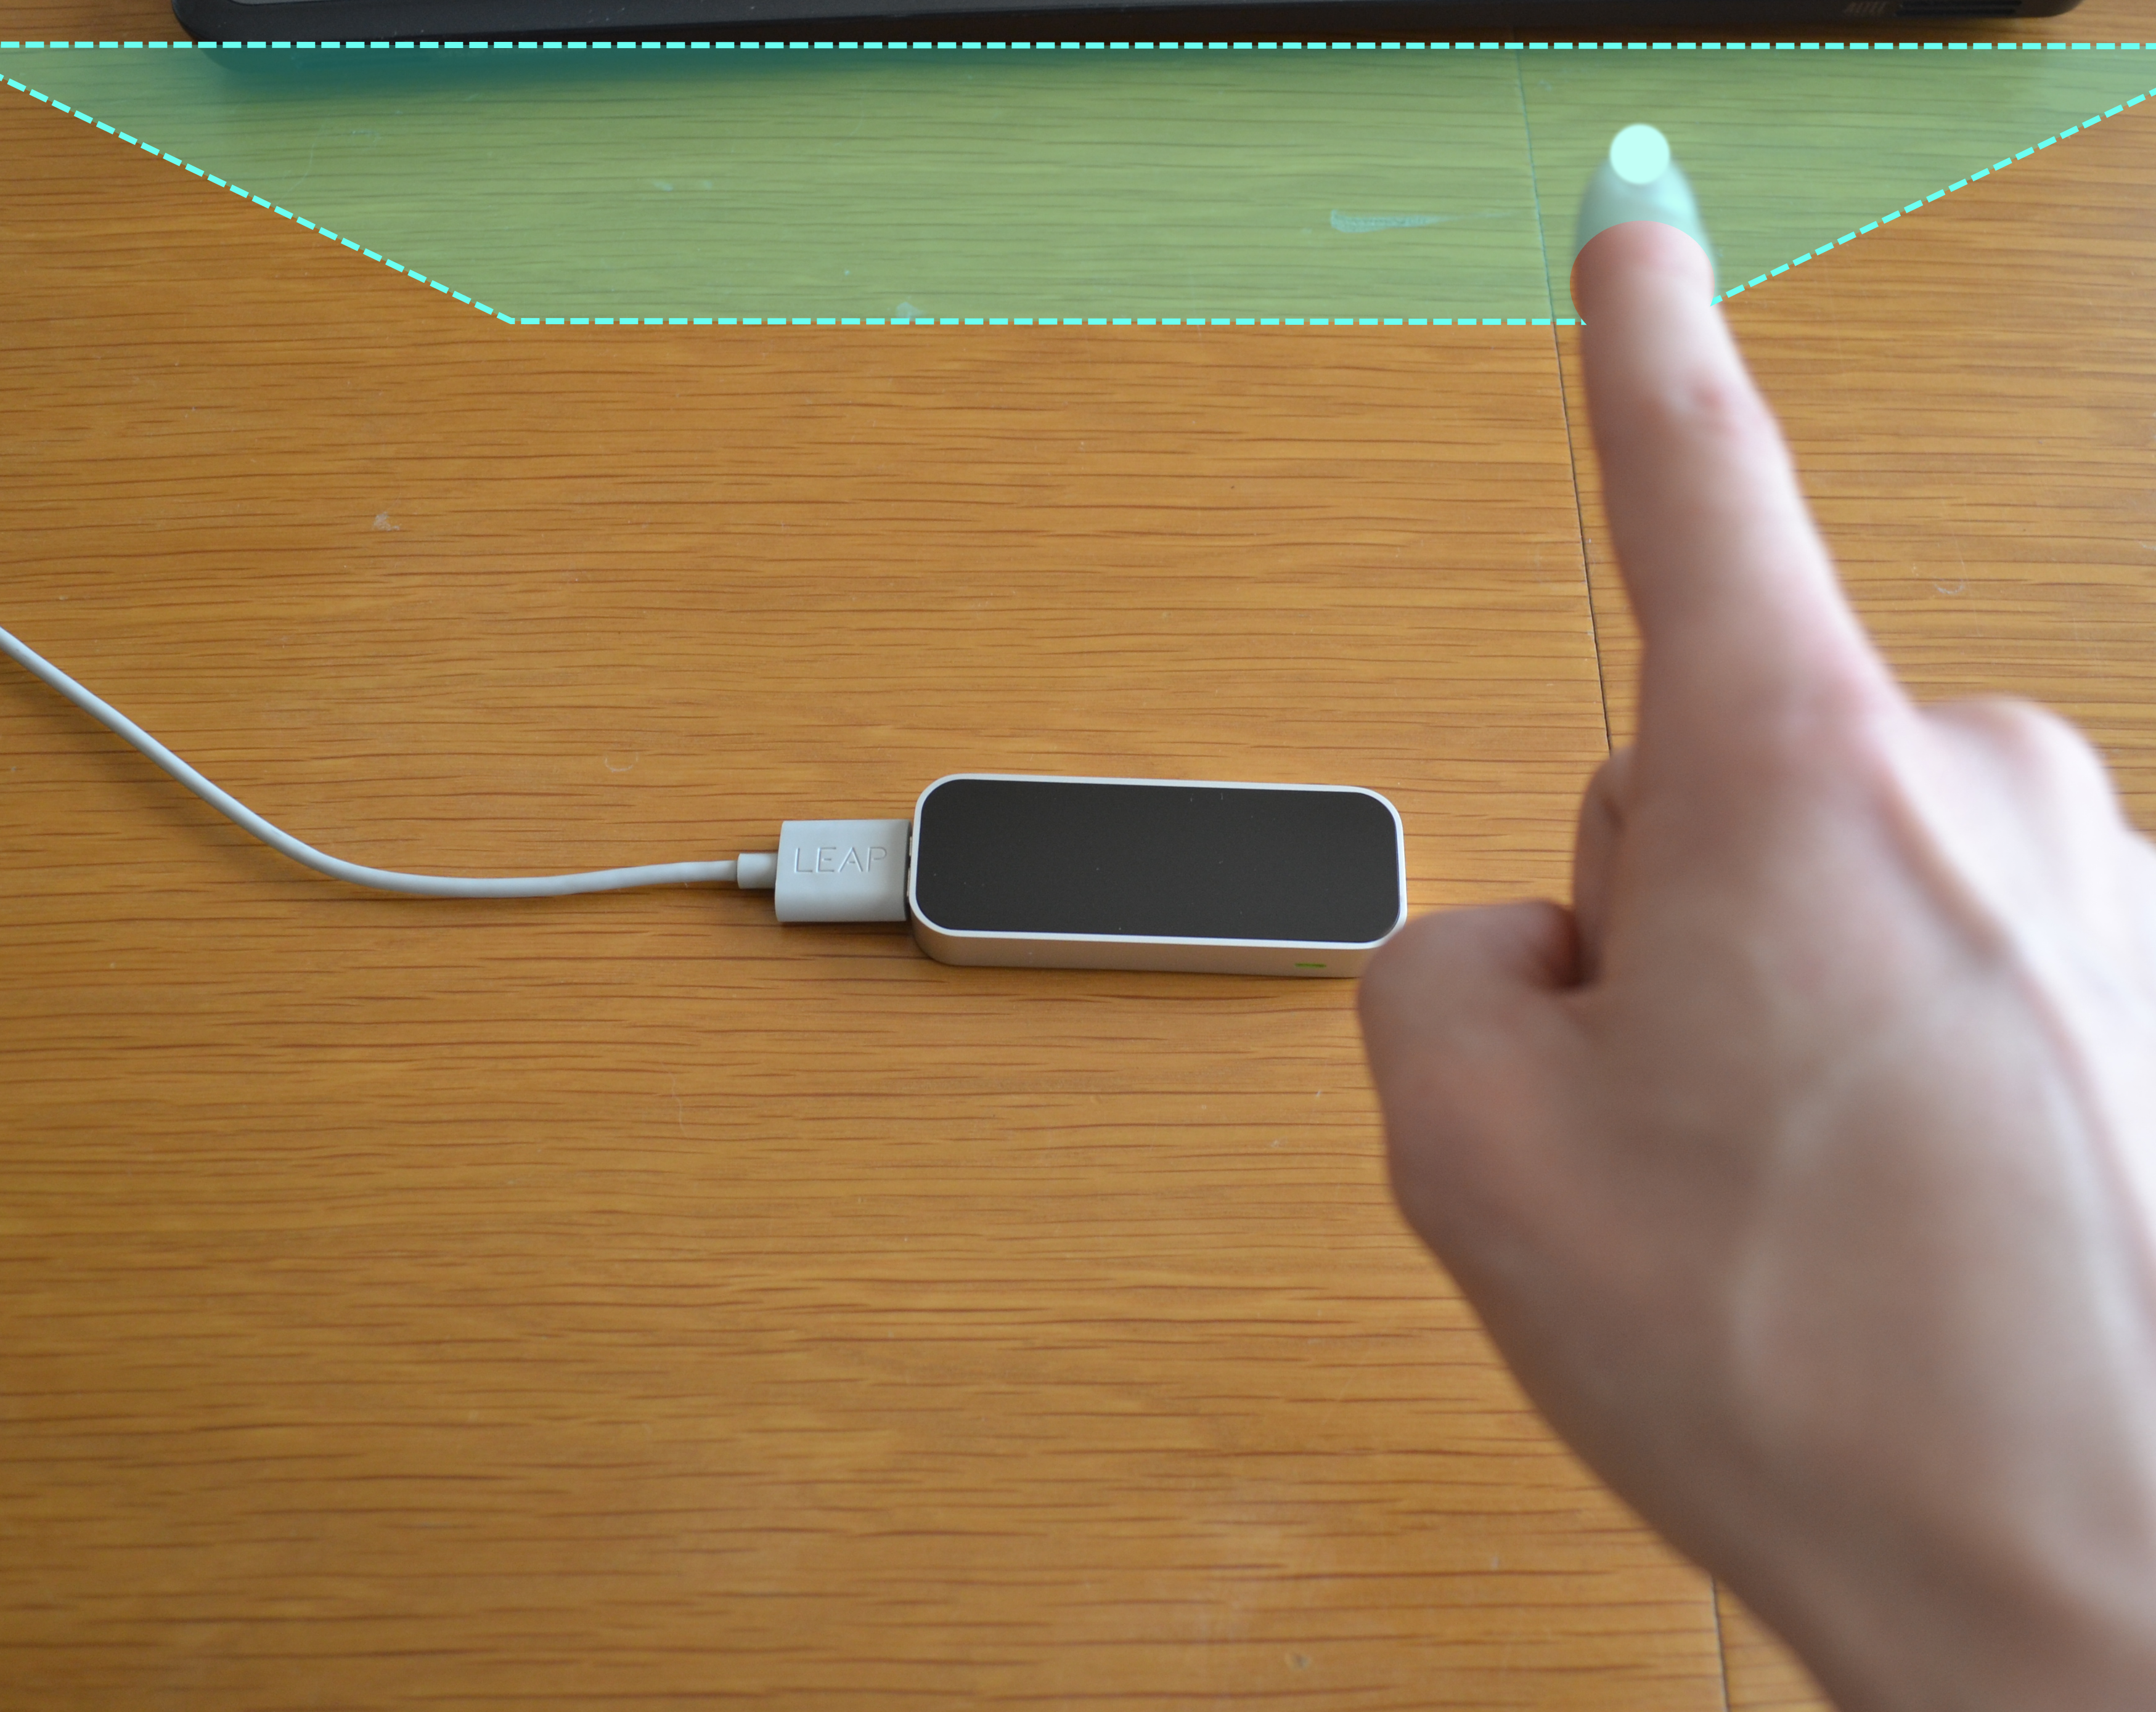
\includegraphics[width=2.5in]{Figures/fig_skimming_before}
		\subcaption{Pressing Key}
	\end{minipage}
	\begin{minipage}[t]{2.5in}
		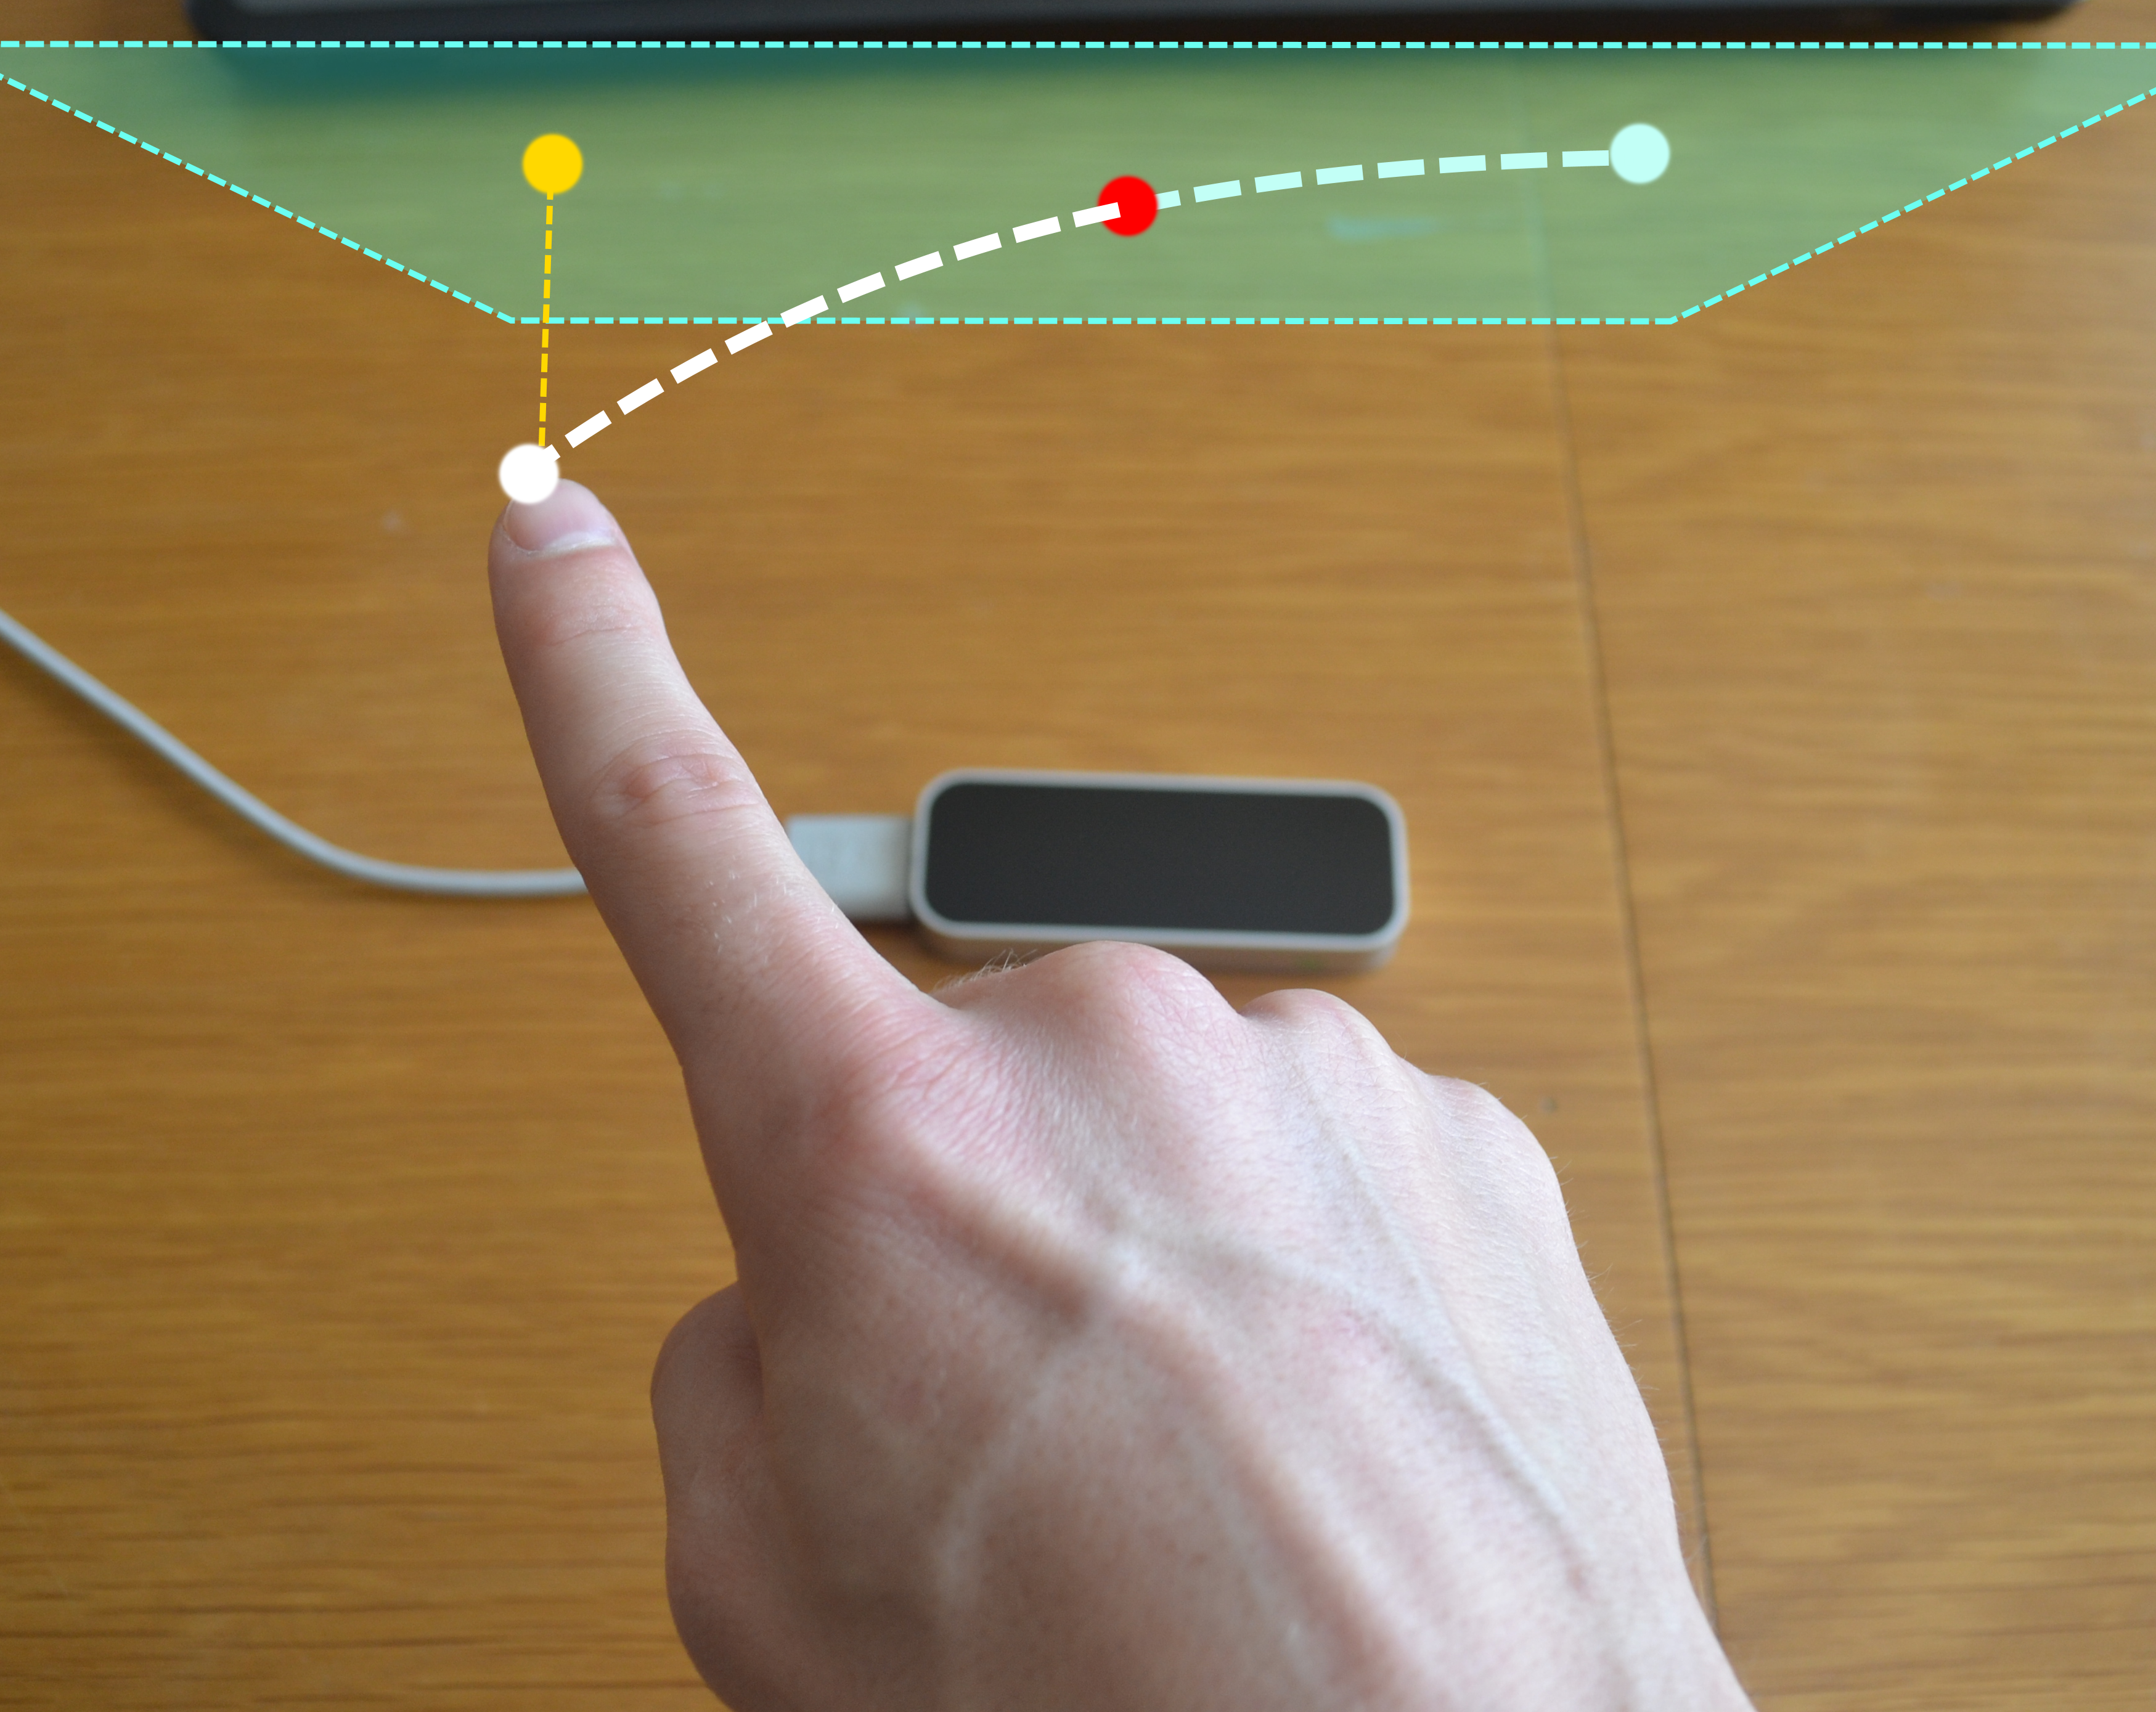
\includegraphics[width=2.5in]{Figures/fig_skimming_after}
		\subcaption{Moving to next Letter across Keyboard}
	\end{minipage}
	\caption[``Skimming'' Problem]{Example of how the natural arcing motion of the arm loses touch as moving across the interaction plane. (a) shows the user pressing a key; and (b) shows the intended destination in \textit{yellow} and the accidental release in \textit{red}.}
	\label{skimming_problem}
\end{figure}

The Leap Surface Keyboard utilized the Static-air implementation to project a mid-air keyboard onto flat surfaces, simulating a touch screen. It's interesting to note that the Leap Surface was essentially indistinguishable from the Touch Screen Keyboard in terms of performance and text-entry rate, reaching 17.1 WPM for a single session. The Leap Surface Keyboard handily proves how essential it is to avoid decoupling the motor space and display space. This implies that the Static-air Keyboard may substantially benefit from an input plane displayed using augmented reality, re-coupling the motor space and display space.

\subsection{Bimodal Interaction}
Bimodal mid-air interactions were shown to be very promising in this thesis and it should be noted that any other secondary input could be used as the source for touch simulation. The Bimodal-air Keyboard reached a text-entry rate of 15.8 WPM for a single session, which was a significant improvement over using pinching or utilizing the 3rd-dimension. The Bimodal-air Keyboard reached 81\% of the text-entry rate of direct touch input and was also often indistinguishable from the Touch Screen Keyboard for many other dependent measures, as detailed in Chapter~\ref{results}. The Bimodal-air keyboard warrants further investigation with a repeated-measures, multiple session study on a traditional word-gesture keyboard implemented with word-recognition.

The Bimodal-air was not without some of its own drawbacks. As with all other mid-air keyboards implemented with the Leap Motion controller, there was an associated input plane that word-gestures were projected onto as the participants moved their hands. This plane, if calibrated or oriented incorrectly, could lead to higher error rates and less precision overall, as seen in Section~\ref{alternative_interaction_plane}.

\subsection{Lacking Word-recognition}
There were some glaring limitations to using a pseudo-implementation of word-gesturing as opposed to using a full word-recognition implementation. A major limitation was that the pseudo-implementation analyzed gestures as they were being created, allowing participants to see real-time updates to path and character production. The software attempted to analyze the current character being pressed based on the deviations in the gesture-path being created and then compared those deviations with the current expected characters. The consequence of this limitation was that participants often interrupted the gesturing process in favor of correcting the erroneous characters, which is absent in traditional word-gesture keyboards that utilize word-recognition. An additional limitation to not analyzing a gesture-shape against a known compendium of common words is the software's increased sensitivity to detecting errors while gesturing, which caused more frequent interruptions of gesture-shapes. This limitation also meant that non-words (e.g., words not in any dictionary) could be produced. Another hindrance was that once an error was made, the likelihood of detecting more errors increased because the path protection would be disabled.

Due to the differences and trade-offs between pseudo-implementation and traditional implementation, it was expected that text-entry rates might have been different than those produced by a traditional word-gesture keyboard applied in mid-air. However, this was not the case. Text-entry rates for a single session with no training were consistent with those produced in Vulture. The Pinch-air keyboard reached a mean text-entry rate of 11.3 WPM as opposed to the mean text-entry rate of 11.8 WPM seen in Vulture \cite{ref_vulture}. This is important because the Pinch-air keyboard was designed to mimic the Vulture technique for word separation.

\subsection{Enforcing Error Correction}
Error correction was enforced due to the higher level of sensitivity to producing errors for the pseudo-implemented word-gesture keyboards. Once one error had been produced, the path protection described in Section~\ref{design} would be disabled since it could no longer be known what the next action of the participant would be. By enforcing correction, the goal was to ensure that the software could always know the next expected key ``press.'' However, requiring the participants to correct erroneous transcriptions presented its own limitations. By requiring error correction, it was much more difficult to track and interpret results for error rates. It is important to note that because participants were required to correct the erroneous transcriptions, the text-entry rates reported in Section~\ref{results_text_entry_rate} were achieved with a 0\% error rate for Vulture's Minimum Word Distance formula \cite{ref_vulture}.


\section{Future Work}
\subsection{Word-recognition}
A future path of this work should use a traditional word-gesture keyboard implementation with word-recognition. This single change will give improved and more standardized results for all measures. Traditional word-recognition would eliminate this thesis's need for enforced error correction, which resulted in modified variables and character-level error production. Because participants would not be distracted with error production mid-gesture, an increase in text-entry rates is expected.

\subsection{Task Redesign}
The task needs to be substantially redesigned to fit a word-recognition implementation of the word-gesture keyboards. First, it would be beneficial to build phrases containing similar gesture-shapes instead of single words to better track text-entry and error rates. Next, there should not be any requirement to correct erroneous words; it should feel natural for the participant and they should fix errors where they feel it is necessary. Finally, the number of trials needs to be increased by a significant amount and extended for repeated sessions so that the true potential of the keyboards' (especially the Bimodal-air's) text-entry rates can analyzed. If implemented on a traditional word-gesture keyboard in mid-air, with repeated sessions and training, the Bimodal-air keyboard is expected to achieve text-entry rates superior to those found in Vulture.

\subsection{Augmented Reality}
Augmented reality would decrease the mental coupling between the gesture motor space and the keyboard display space, and therefore would be a huge boon for 3-dimensional mid-air implementations. This is theorized to benefit the Static-air Keyboard most due to the success of the Leap Surface Keyboard, which is simply the Static-air keyboard projected onto a surface. Participants being able to directly see the mid-air keyboard they are using would be expected to substantially increase text-entry rates.

\subsection{The ``Skimming'' Issue}
The simplest way to solve the ``skimming'' issue is to increase the interaction plane's release threshold. As shown in Figure~\ref{skimming_problem_fix}, once a simulated touch has been made, increasing the release threshold toward the participant so that the participant's hand does not leave the interaction plane when moving on the $x$ and $y$ axes. This change is expected to reduce accidental releases and improve results for the Static-air Keyboard. A similar approach could also be used for the Predictive-air Keyboard because quick side-to-side movements were sometimes seen as a touch being released.

\begin{figure}[!t]
	\centering
	\begin{minipage}[t]{2.5in}
		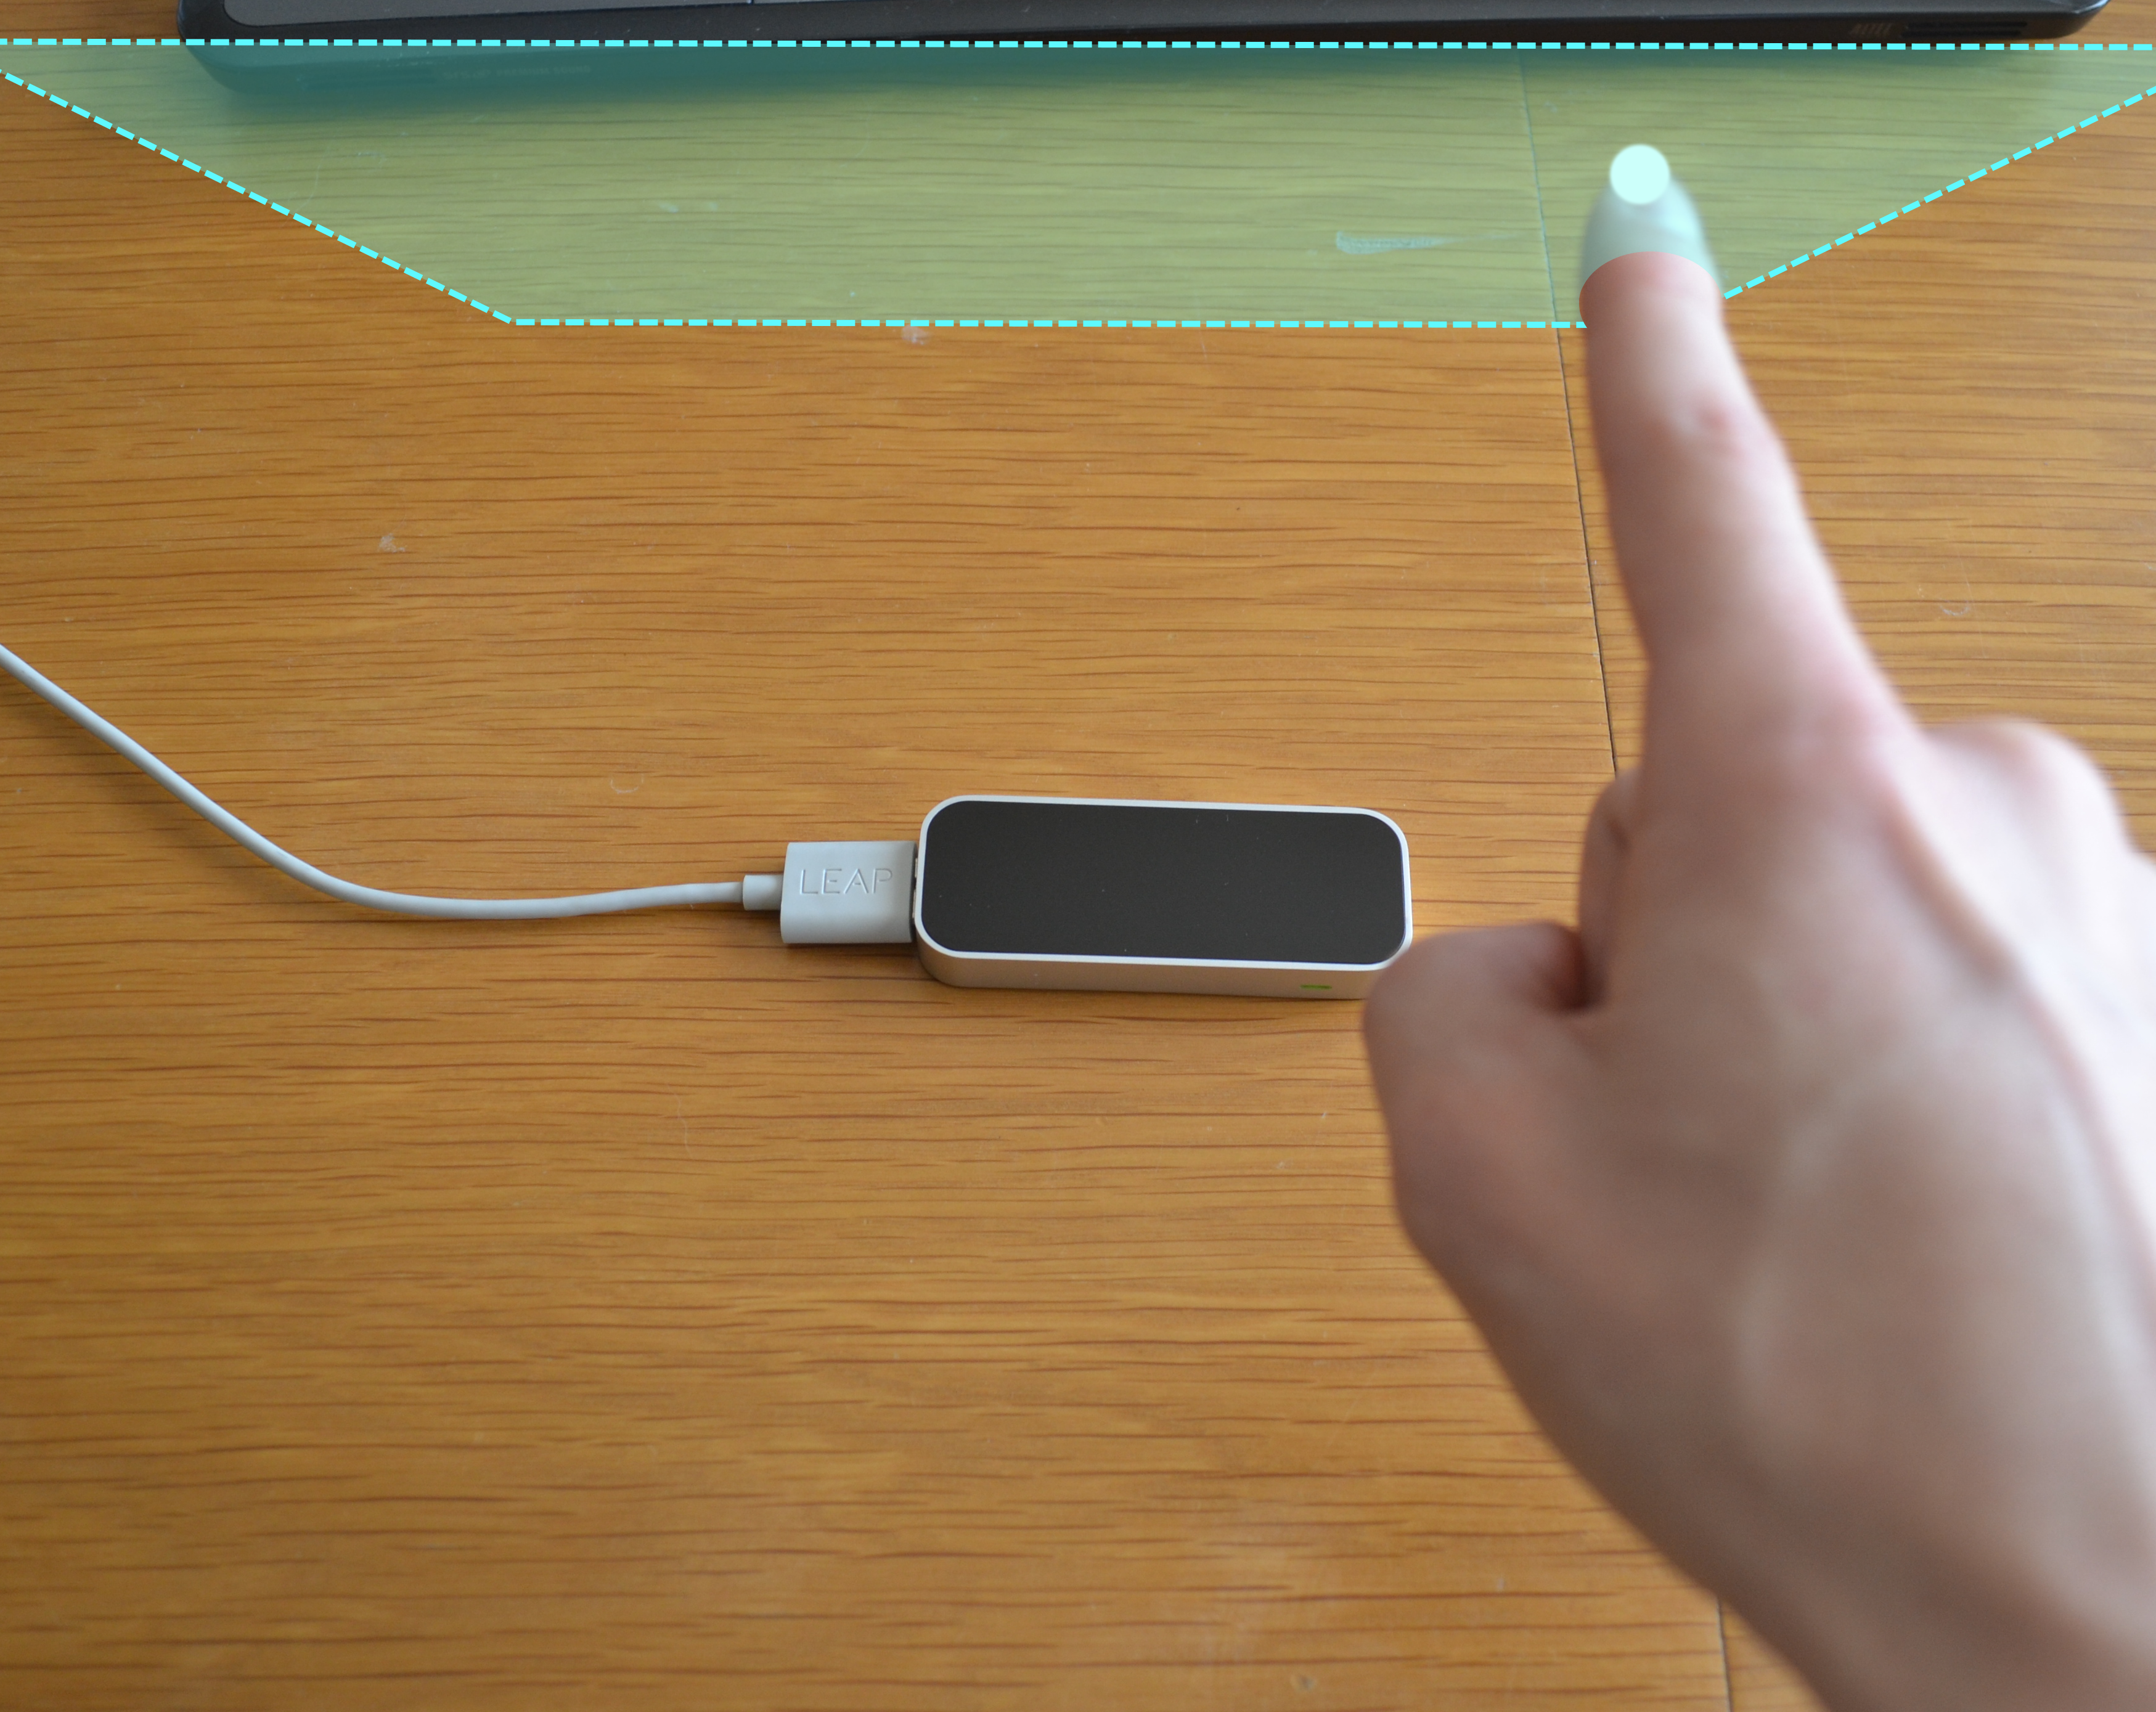
\includegraphics[width=2.5in]{Figures/fig_skimming_fix_before}
		\subcaption{Intersecting Plane to hit First Key}
	\end{minipage}
	\begin{minipage}[t]{2.5in}
		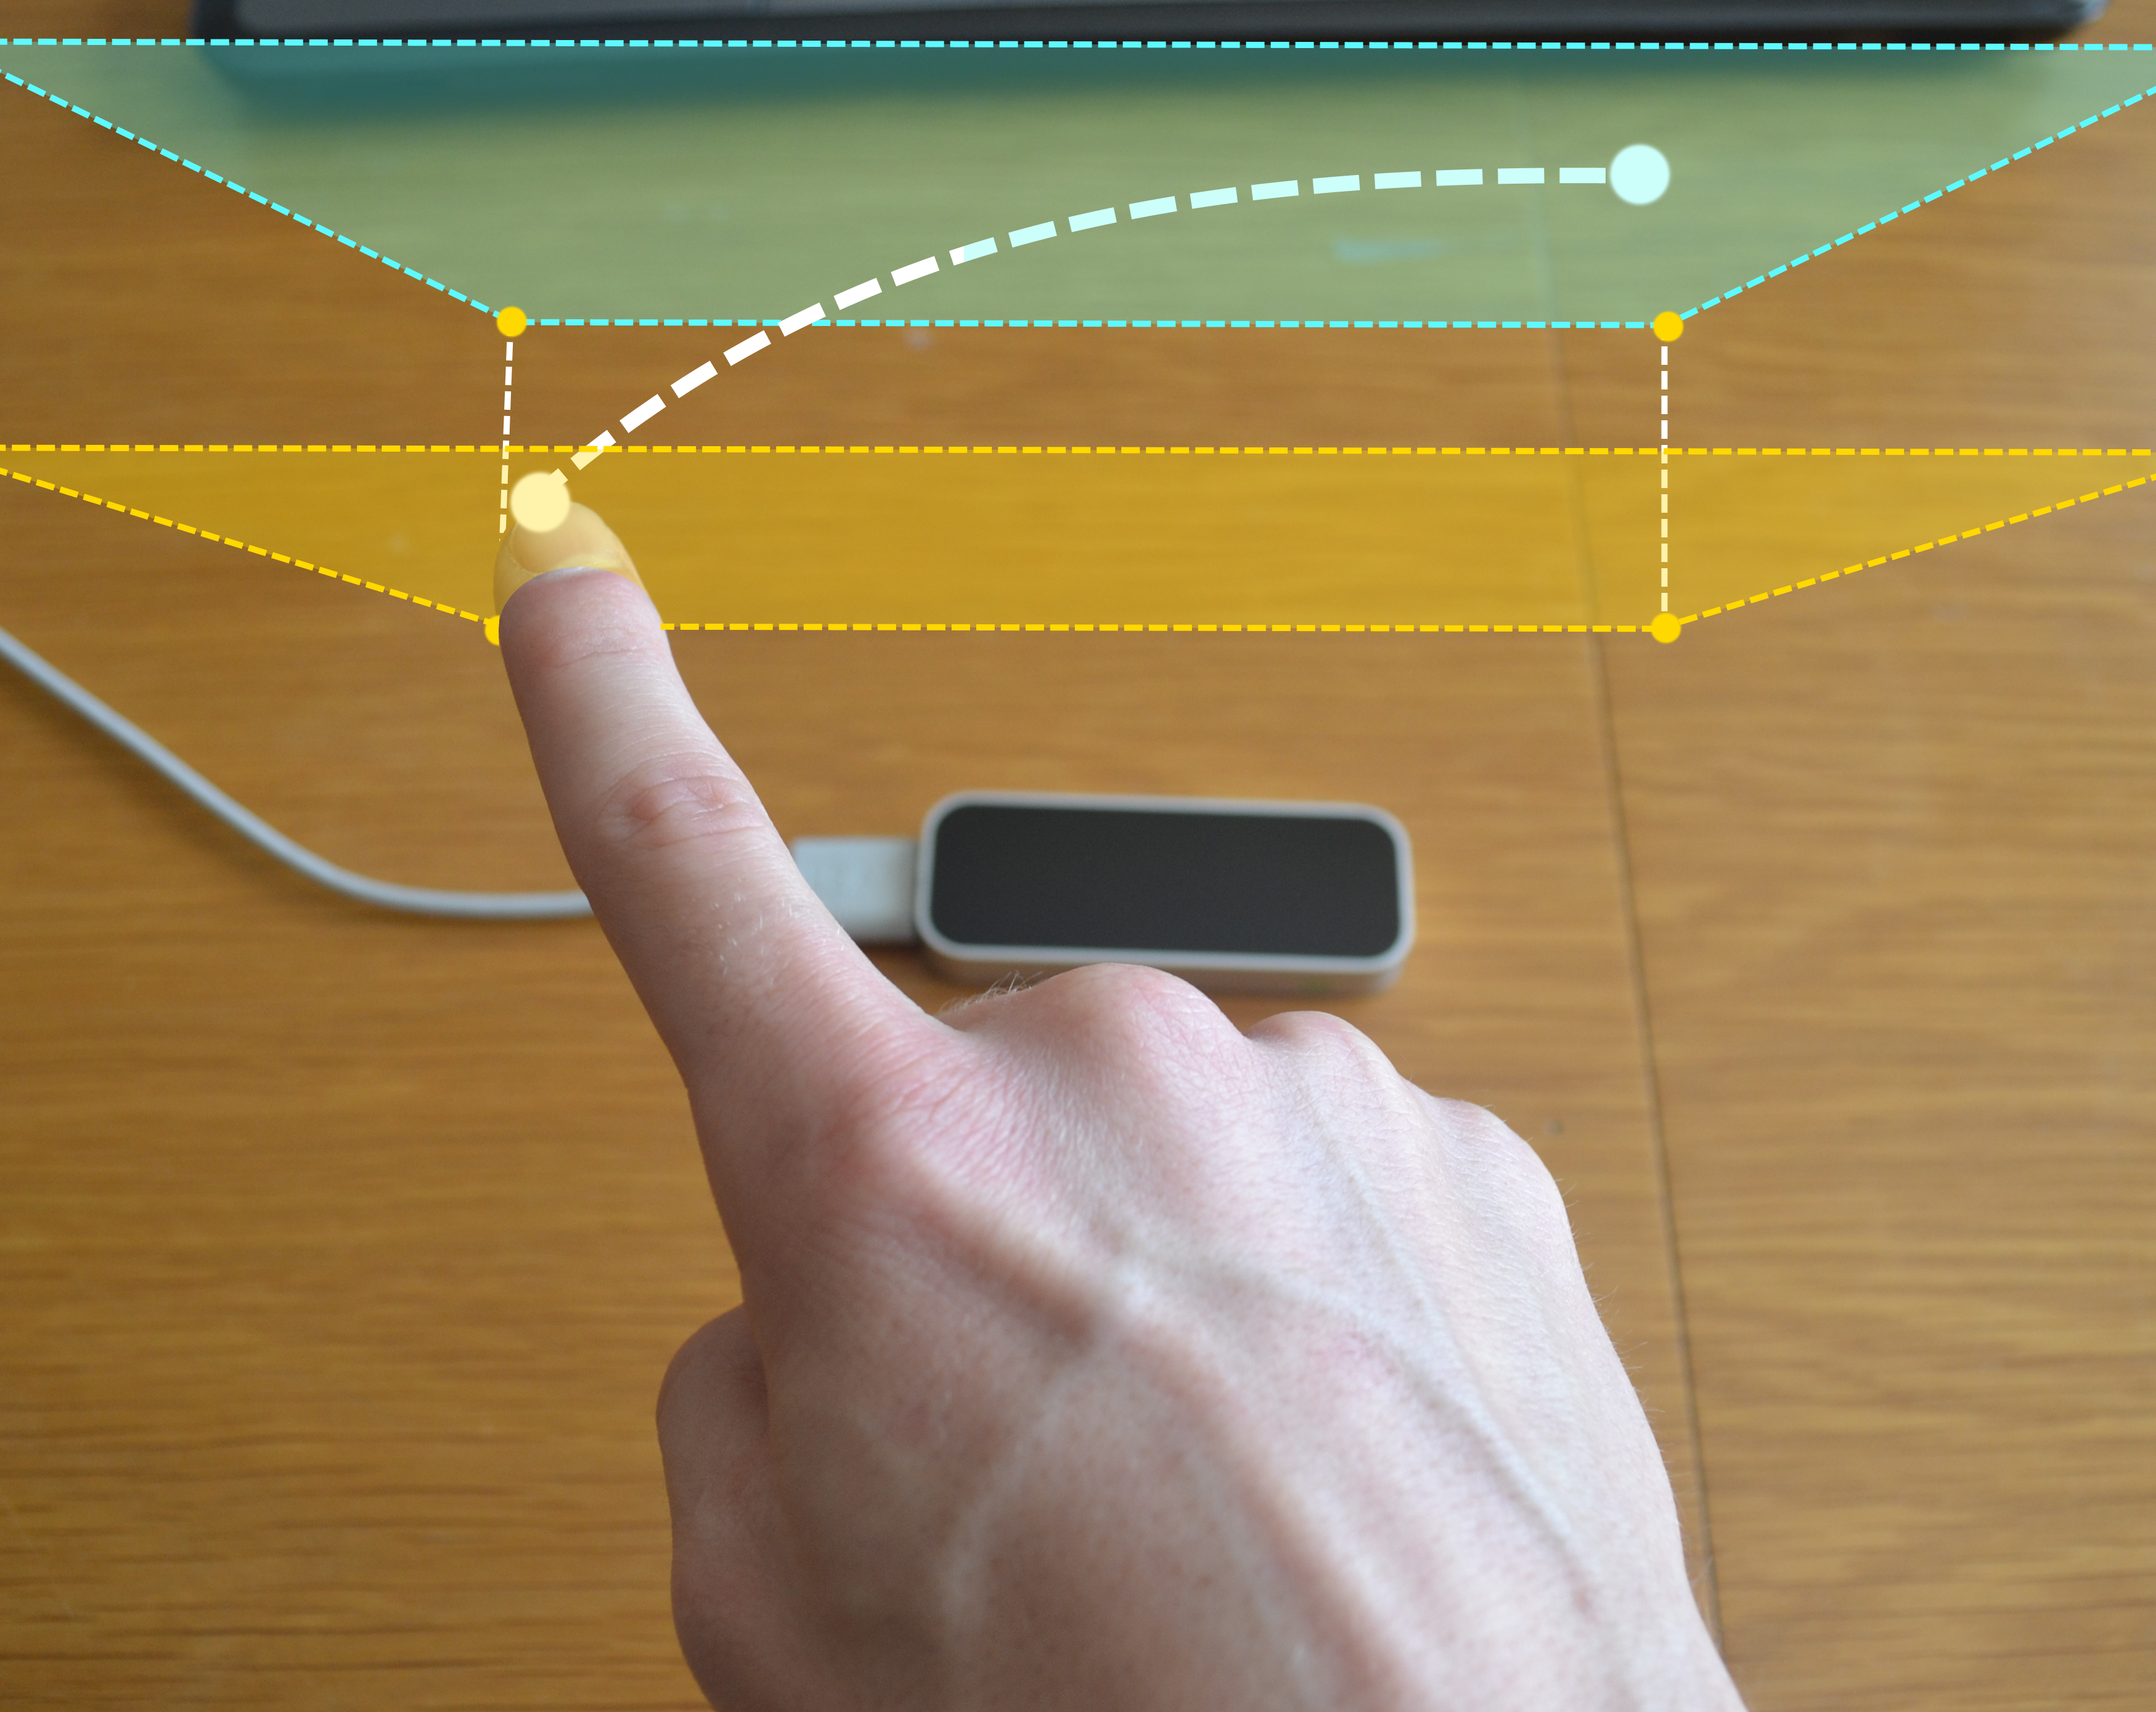
\includegraphics[width=2.5in]{Figures/fig_skimming_fix_after}
		\subcaption{Increased Release Threshold}
	\end{minipage}
	\caption[``Skimming'' Solution]{An example of how the ``skimming'' issue could be fixed by increasing the release threshold after touching. (a) shows the user pressing the first key; and (b) shows the increased release threshold for the interaction plane as the user moves across to the next key.}
	\label{skimming_problem_fix}
\end{figure}

\subsection{Improved Tracking}
During the study, the Leap Motion controller often had issues detecting participants' pointer fingers or palms. A major factor of these detection issues was due to the positioning of the Leap Motion controller itself, as well as some participants holding their hand in an upward position, as shown in Figure~\ref{finger_blocked}. A simple solution to this issue is to angle the Leap Motion controller so that it is facing the participant at an angle providing a wider range of view, as seen in Figure~\ref{finger_seen}.

\begin{figure}[!t]
	\centering
	\begin{minipage}[t]{2.5in}
		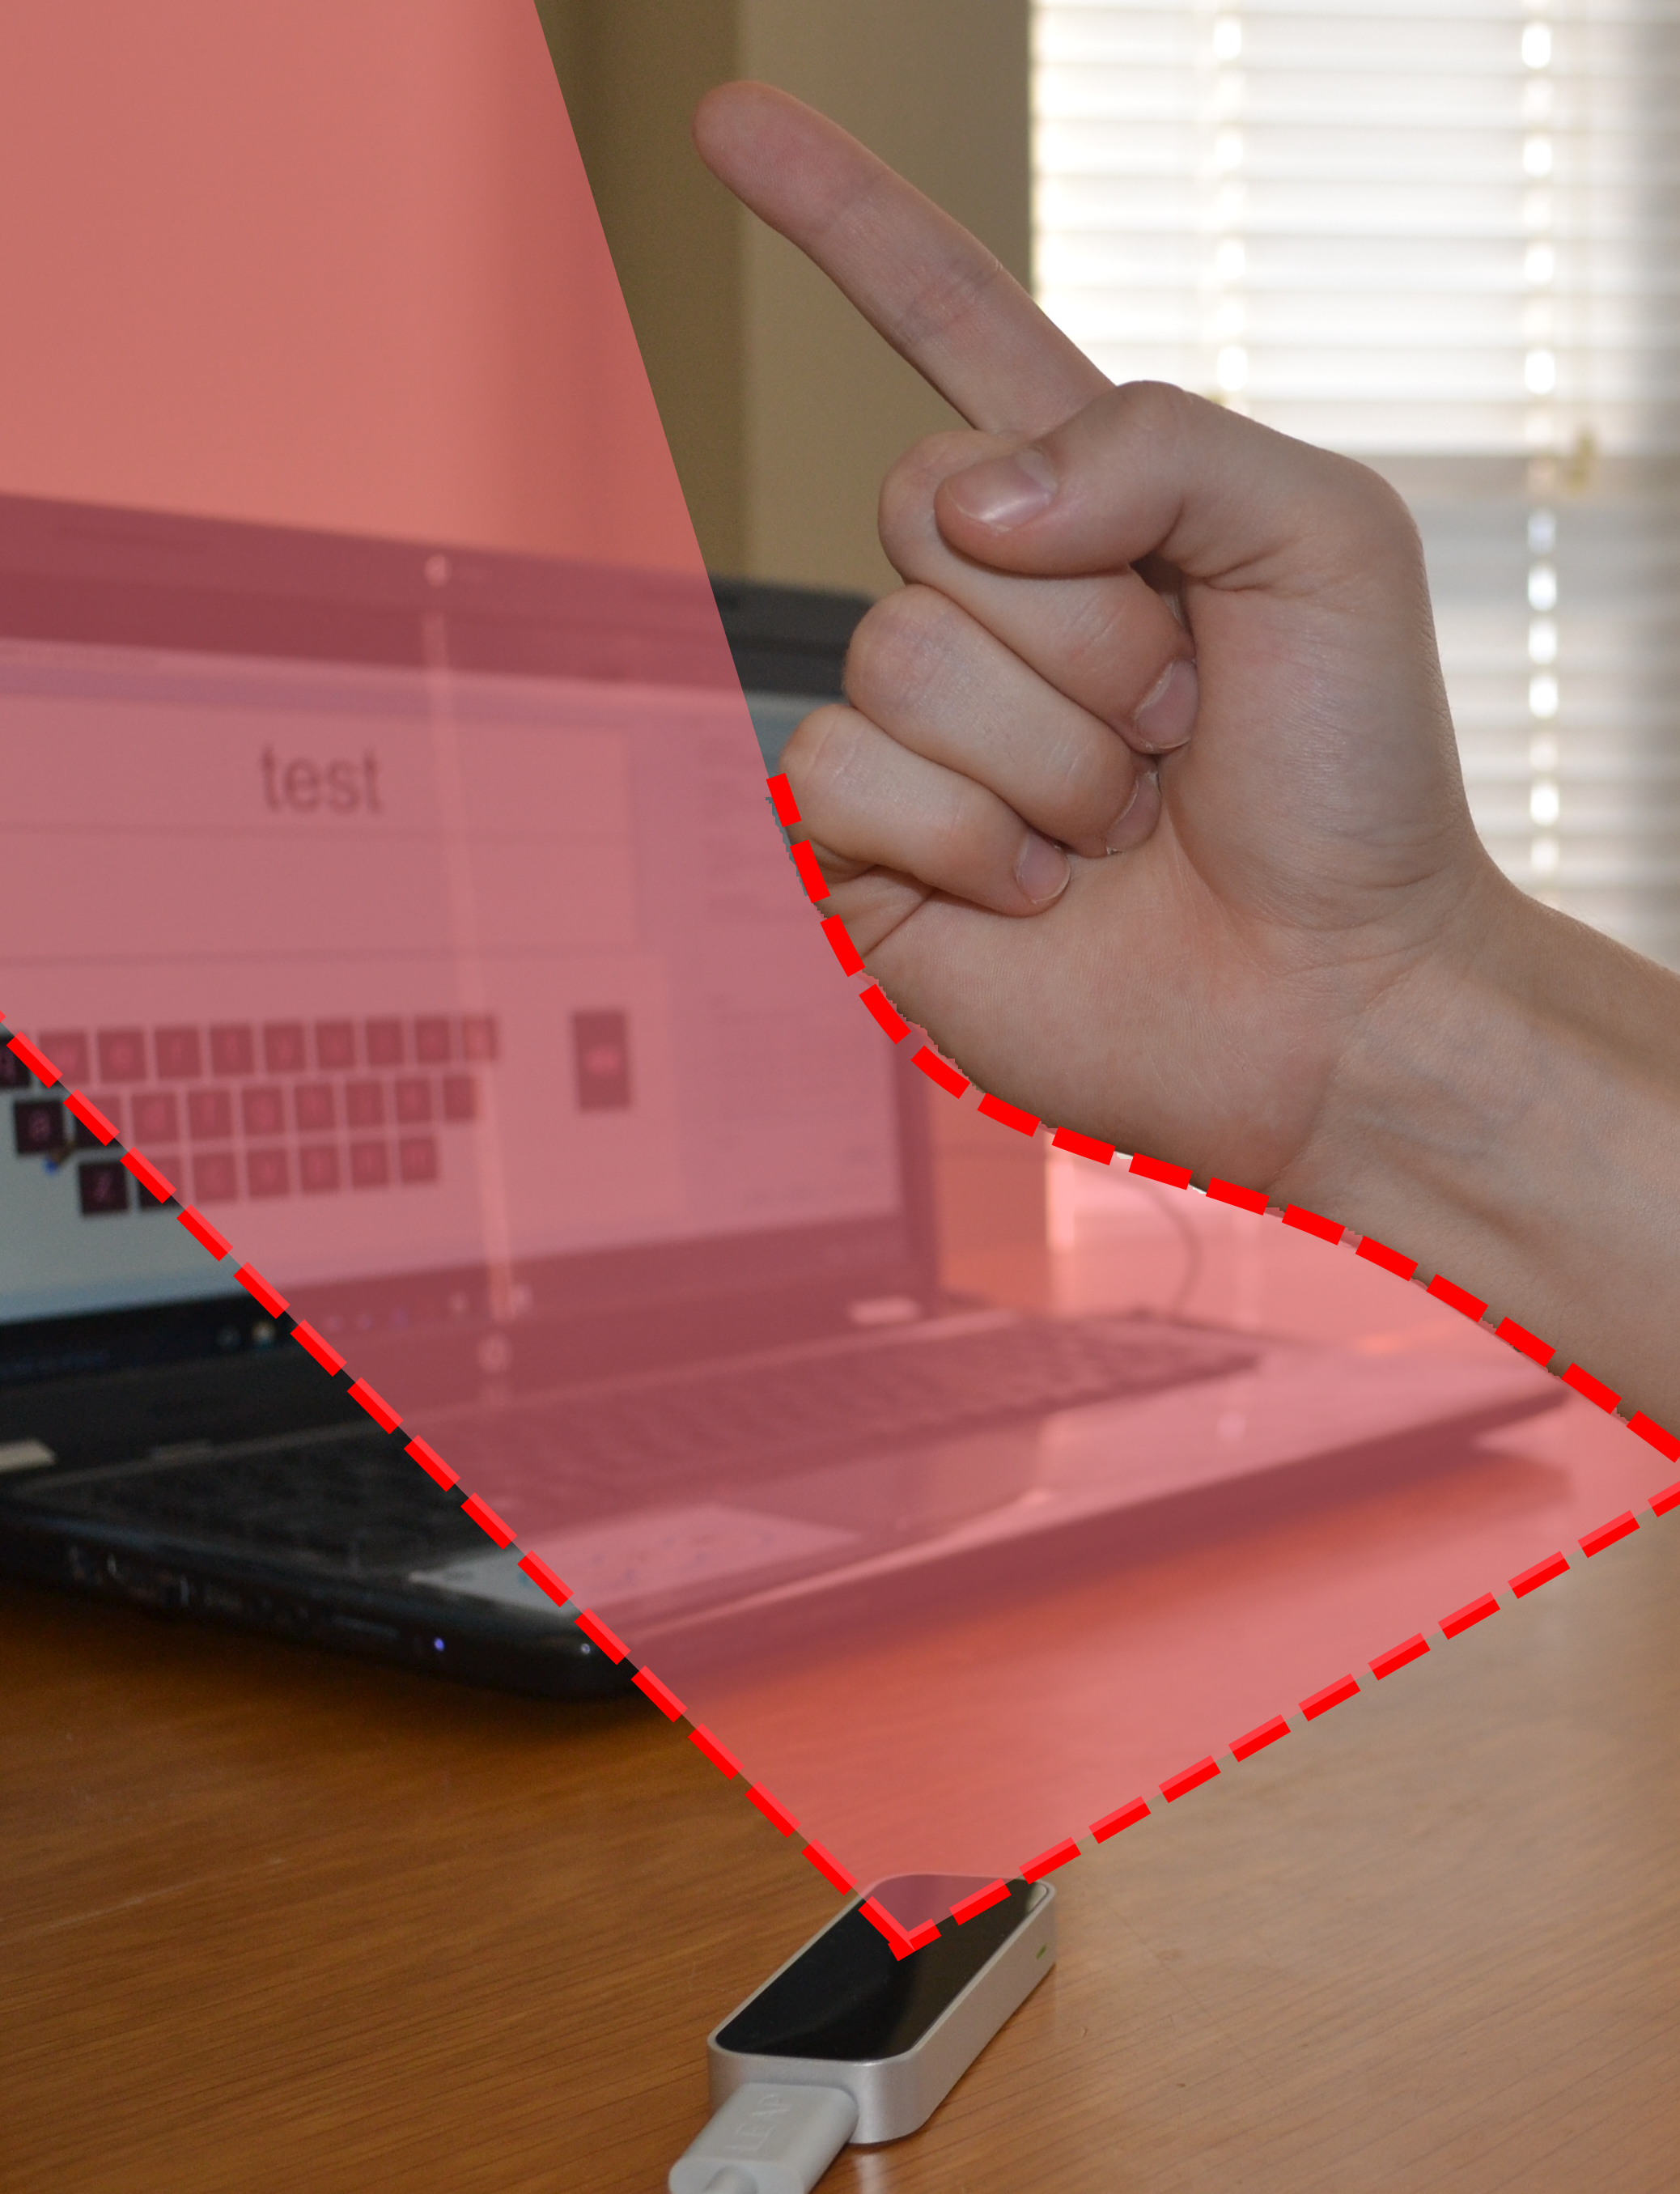
\includegraphics[width=2.5in]{Figures/fig_blocking}
		\subcaption{Hand Blocking Finger}
		\label{finger_blocked}
	\end{minipage}
	\begin{minipage}[t]{2.5in}
		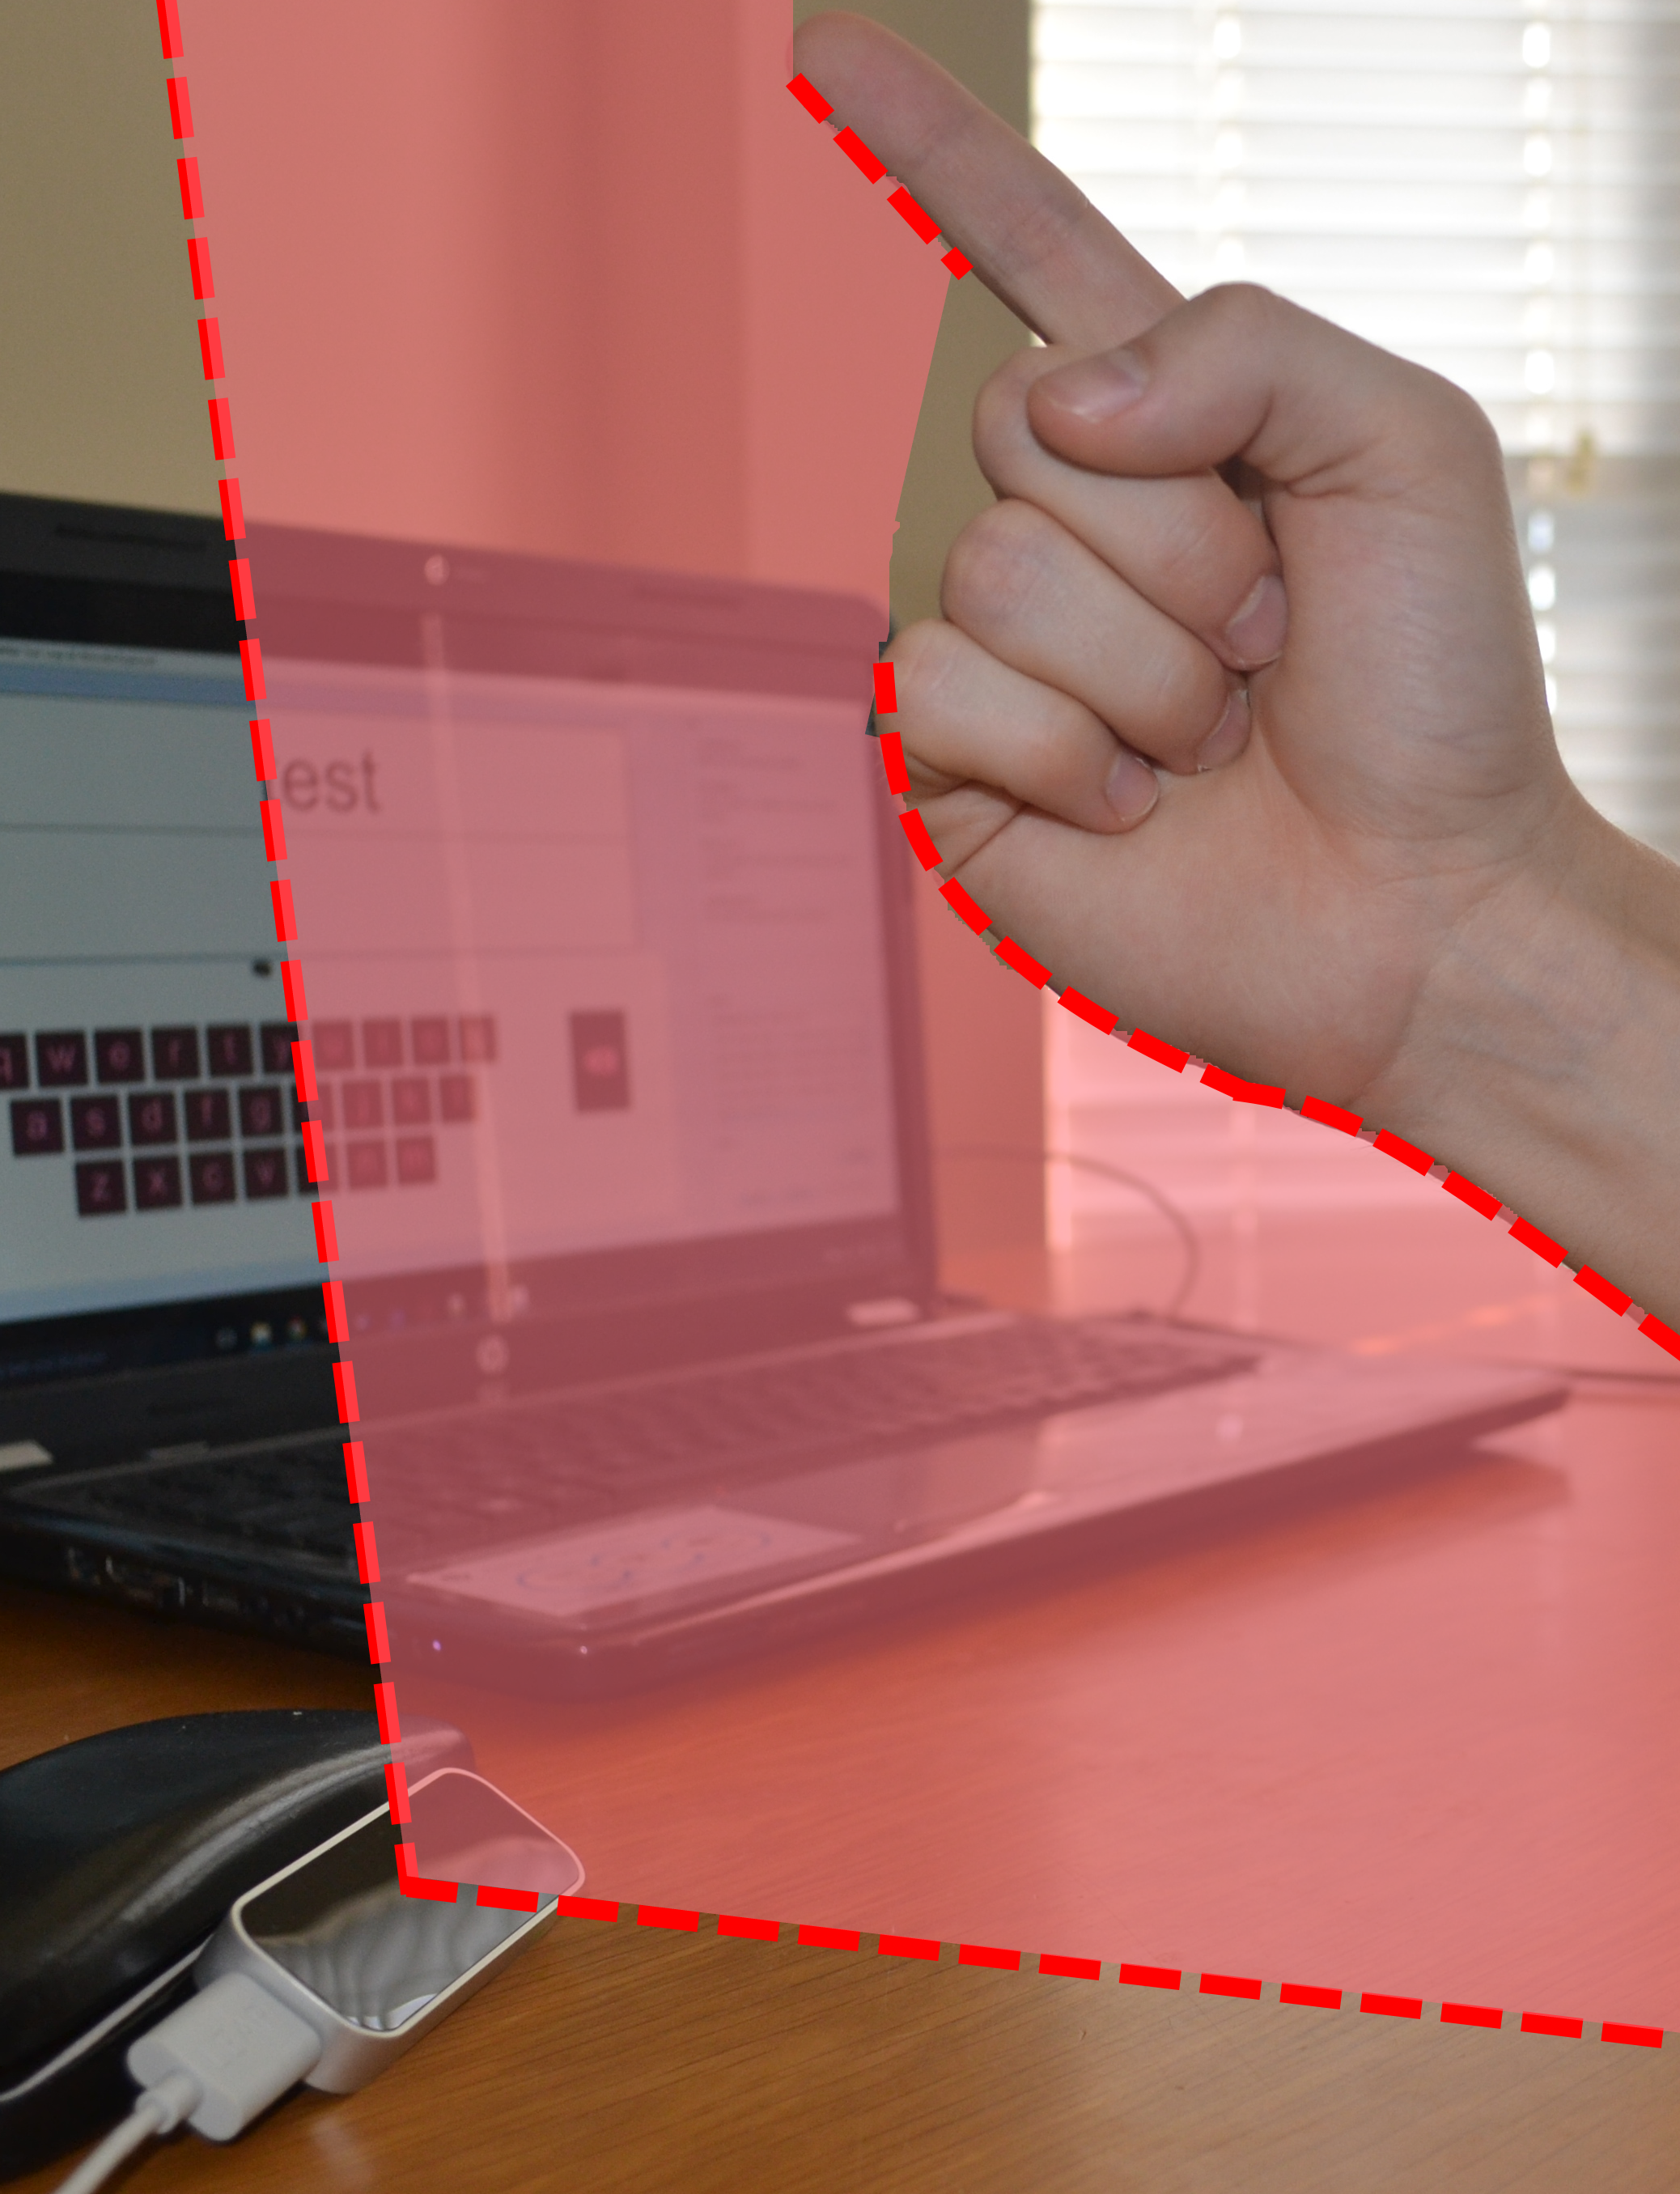
\includegraphics[width=2.5in]{Figures/fig_angled}
		\subcaption{Angle Reveals Finger}
		\label{finger_seen}
	\end{minipage}
	\caption[Blocking Problem]{Examples of how some participants blocked their finger from being tracked. (a) shows the user blocking the view of their finger with their hand; (b) shows how an angled Leap Motion controller might solve the problem.}
	\label{blocking problem}
\end{figure}

\subsection{Alternative Interaction Plane} \label{alternative_interaction_plane}
As participants moved across the interaction plane in mid-air, sometimes the side-to-side movements and up and down movements were not represented as expected, as seen in Figure~\ref{bad_calib_problem}. Better approaches to calibration and plane-creation, such as those discussed in Personal Space and elsewhere  \cite{ref_alvin_thesis,ref_darren_thesis}, need to be implemented. A spherical or even curved interaction plane designed for each individual participant would greatly benefit all of the mid-air keyboards especially so that participants would be able to rest their arms \cite{ref_darren_thesis}. With a flat, quadrilateral plane, many participants suffered the same issues as mentioned in \cite{ref_alvin_thesis}, especially when moving to the extreme edges of the projected keyboard.

\begin{figure}[!t]
	\centering
	\begin{minipage}[t]{5in}
		\begin{minipage}[t]{1.5in}
			\begin{minipage}[t]{1.5in}
				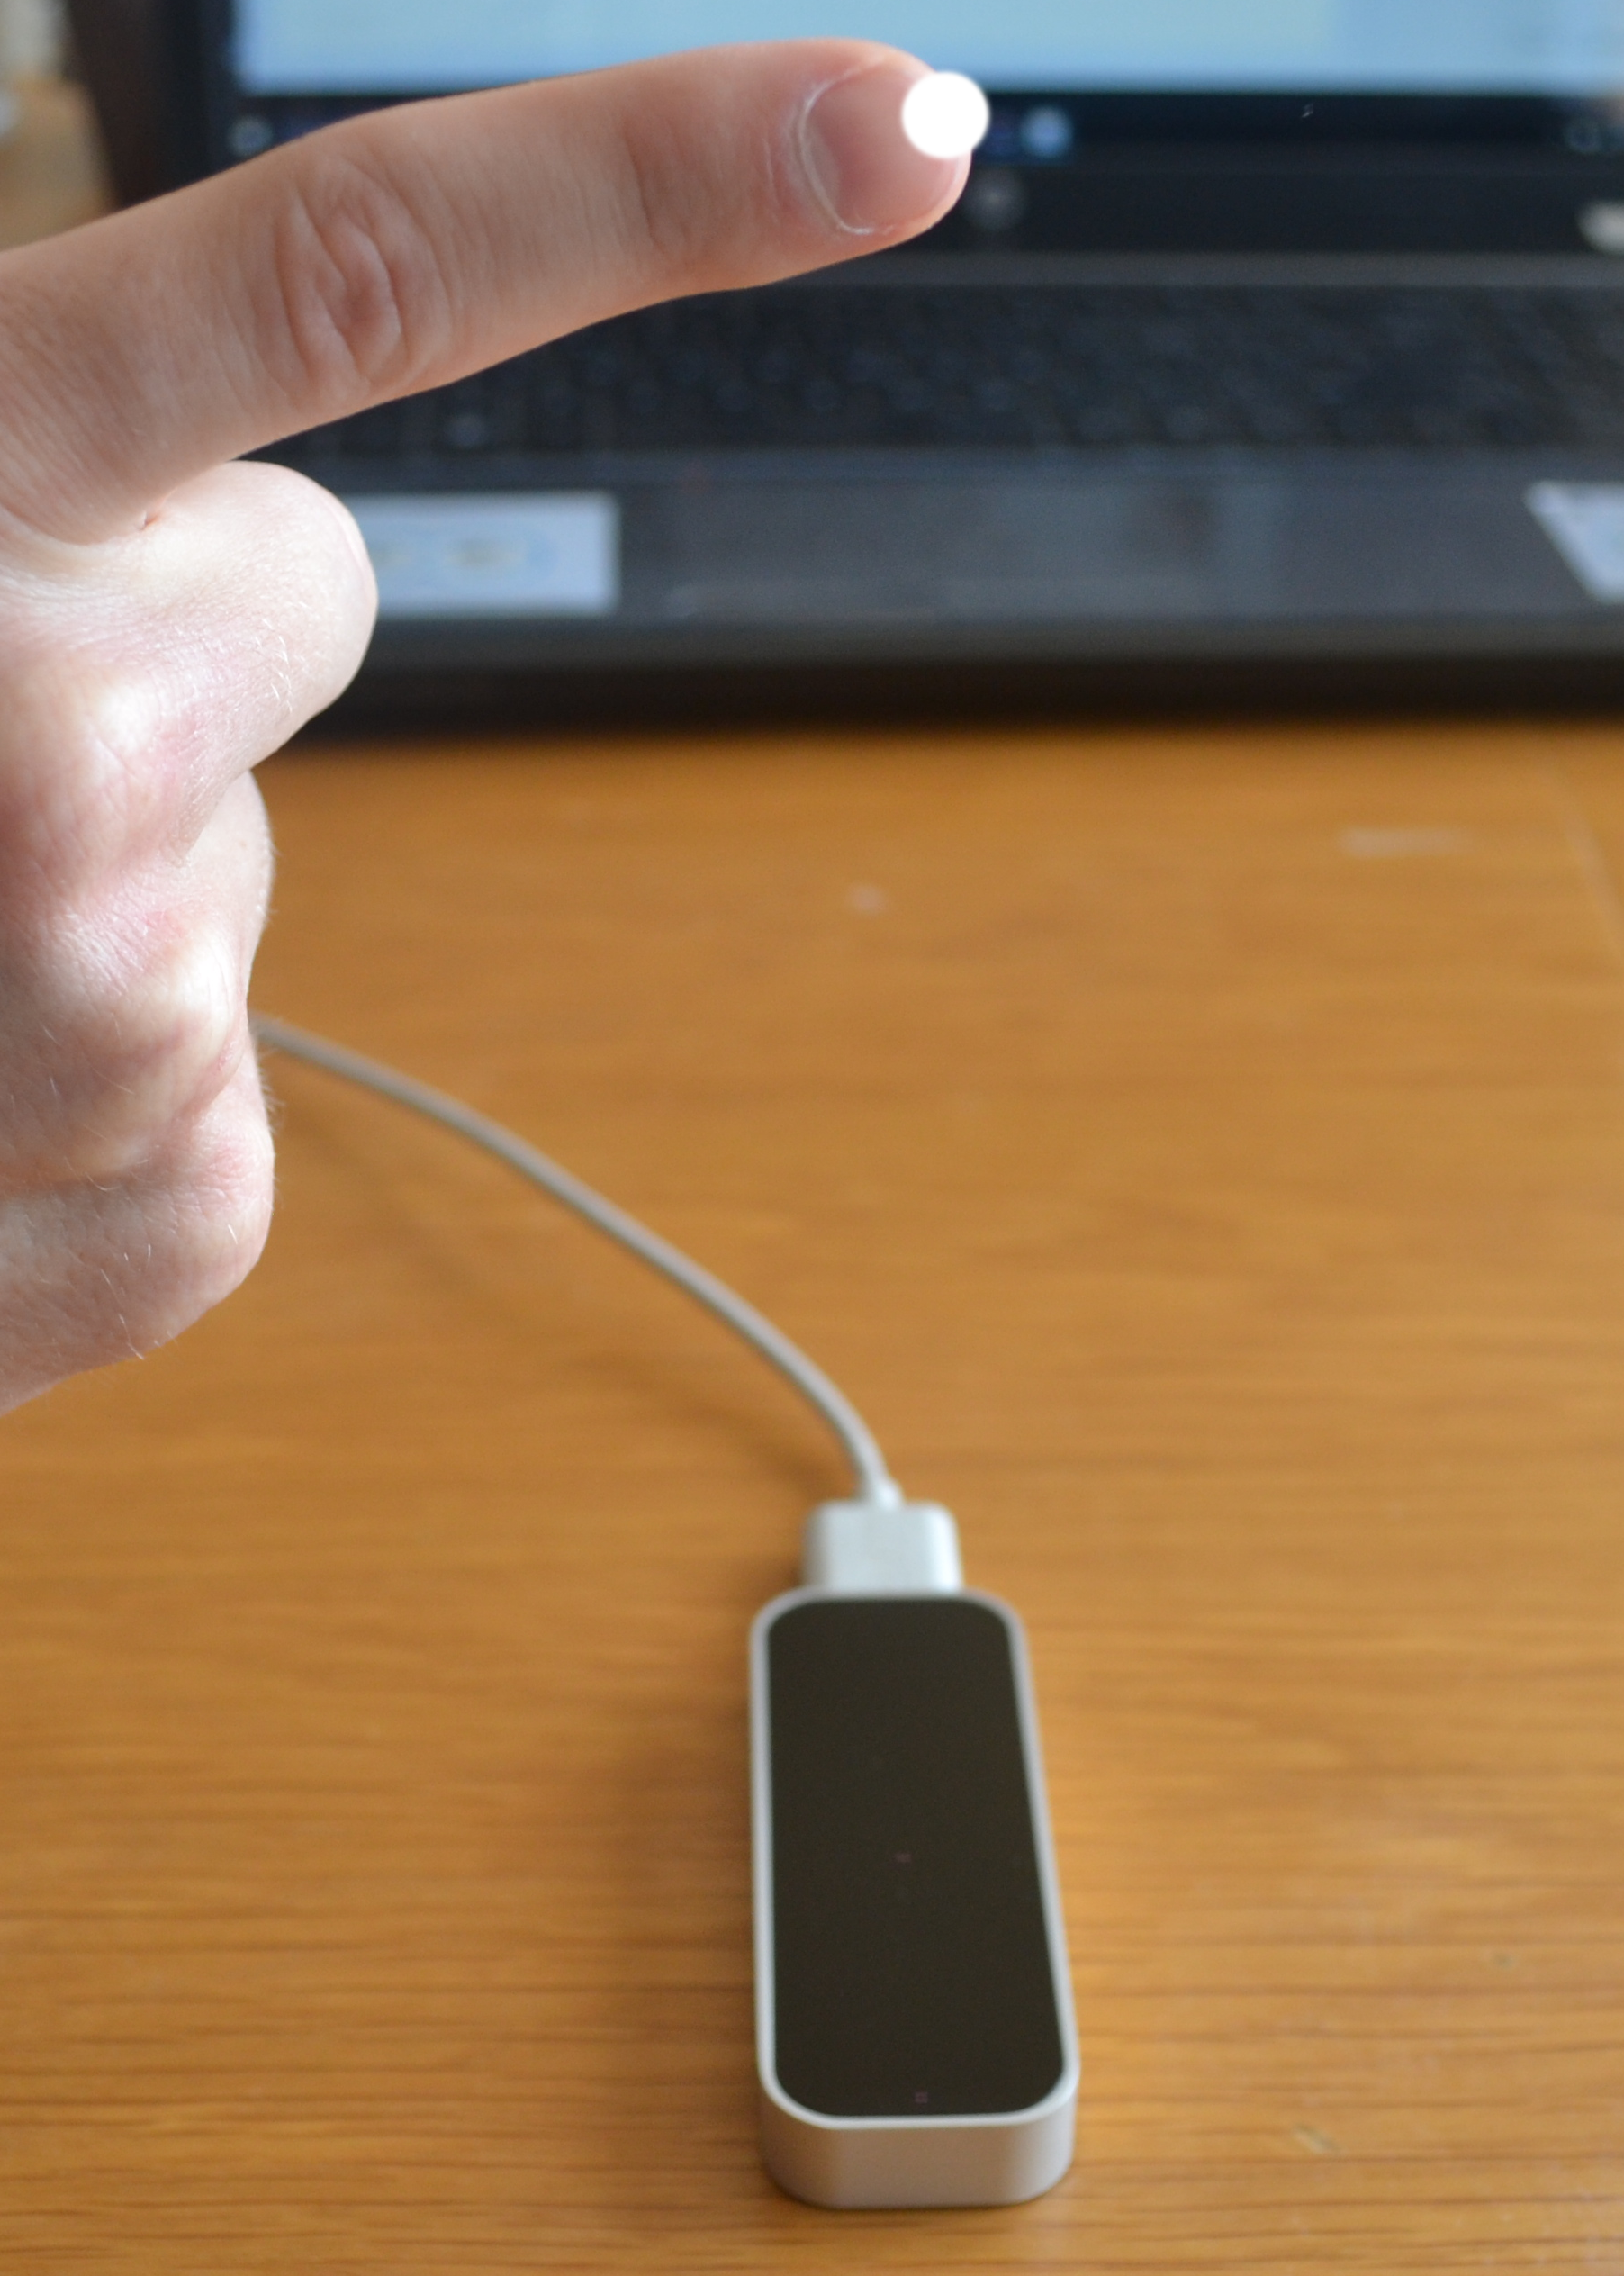
\includegraphics[width=1.5in]{Figures/fig_bad_calib_before}
			\end{minipage}
			
			\begin{minipage}[t]{1.5in}
				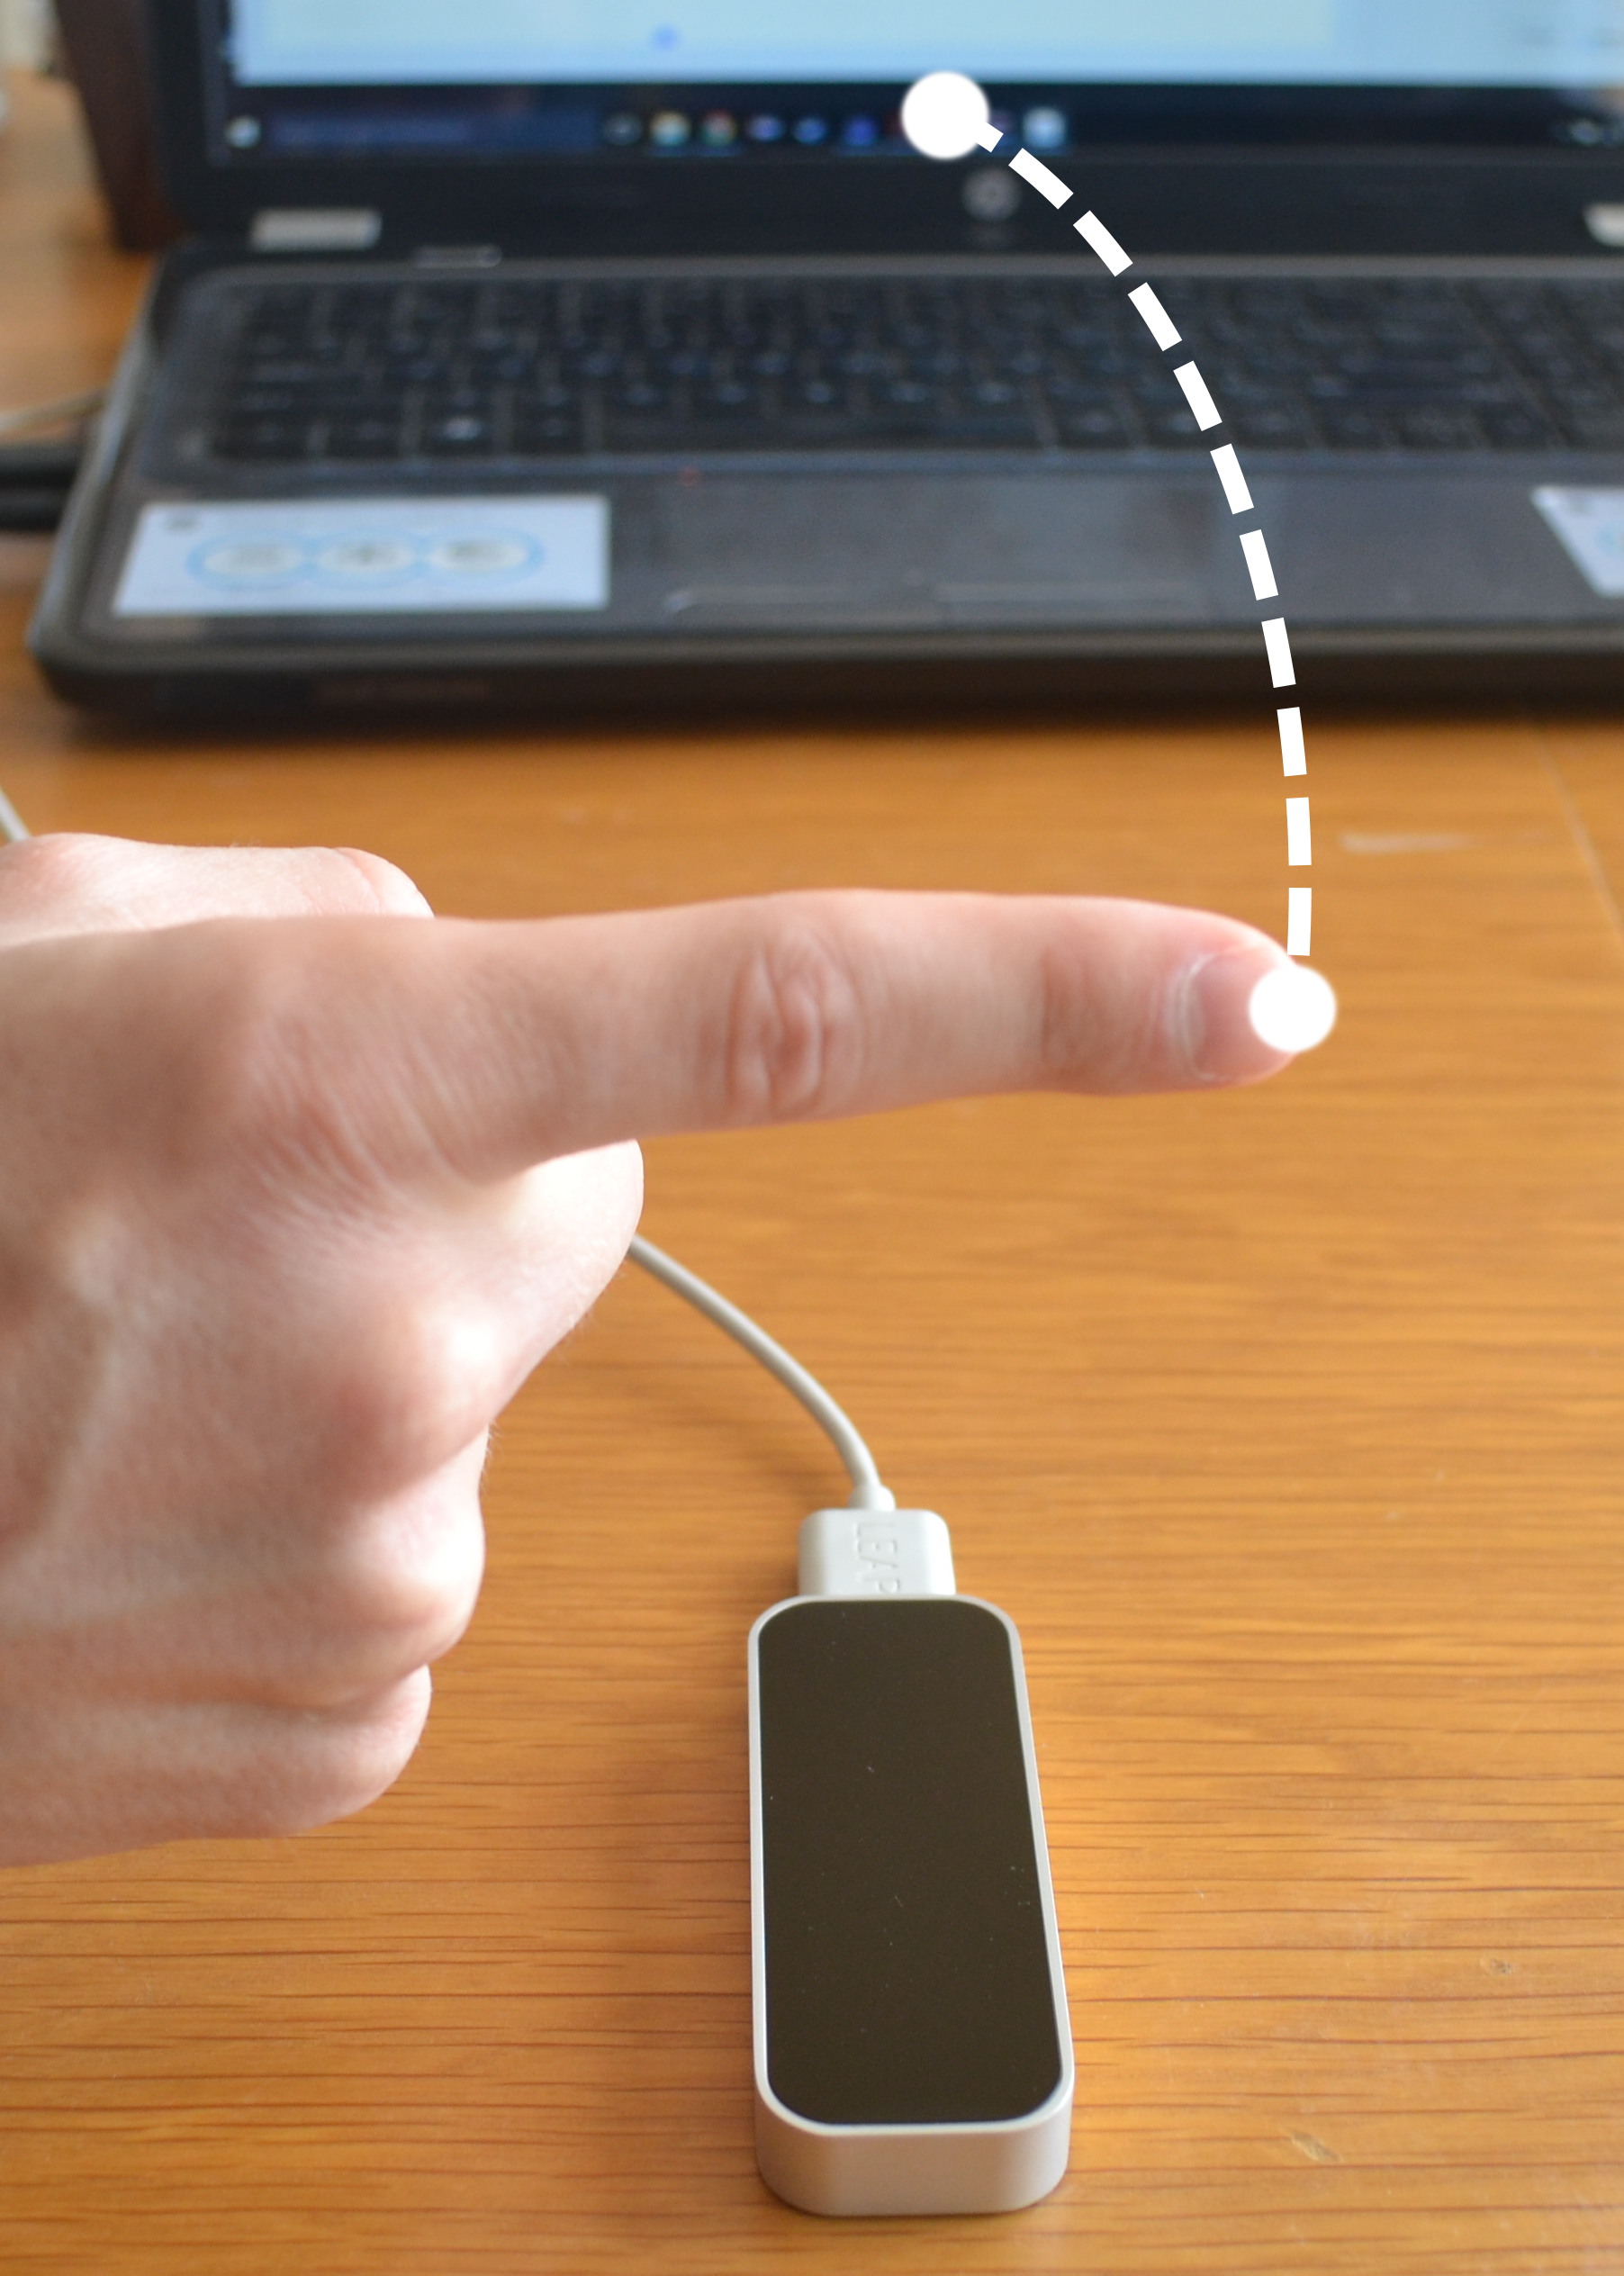
\includegraphics[width=1.5in]{Figures/fig_bad_calib_after}
			\end{minipage}
			\subcaption{Movement}
		\end{minipage}
		\begin{minipage}[t]{3.5in}
			\begin{minipage}[t]{0.4in}
			\end{minipage}
			\begin{minipage}[t]{3.1in}
				\includegraphics[width=3.1in]{Figures/fig_intended_path}
			\end{minipage}
			
			\begin{minipage}[t]{0.4in}
			\end{minipage}
			\begin{minipage}[t]{3.1in}
				\includegraphics[width=3.1in]{Figures/fig_actual_path}
			\end{minipage}
			\subcaption{Intended Path (\textit{Top}) vs. Actual Path (\textit{Bottom})}
		\end{minipage}
	\end{minipage}
	\caption[Bad Calibration Example]{Example showing how a bad calibration affects movement. (a) shows a user trying to make a vertical movement; and (b) shows how the actual path was misaligned because of the calibration and orientation of the Leap Motion controller.}
	\label{bad_calib_problem}
\end{figure}

\subsection{Multi-functional Space}
Since mid-air word-gesturing keyboards utilize the 3rd-dimension or implement a bimodal approach, hand gestures could be used for alternative interactions when not simulating a touch (e.g., control a cursor, make a selection, etc.). This would allow users to fully interact with screens of any kind, including projections, and not limit the user to a keyboard and mouse.

\subsection{Image Processing}
The Leap Surface Keyboard's projected virtual keyboard revealed an area for possible expansion. While the hard-coded software keyboard functioned adequately, image processing could make the feature much more versatile. Being able to print out and use any keyboard for word gesturing or otherwise could be highly beneficial.

\subsection{Gaming Console Keyboards} \label{future_gaming_keyboard}
Using the Xbox Controller Keyboard in the pre-pilot and the pilot study confirmed the inconvenience of single-input text-entry. Therefore, it would be beneficial to apply what has been learned from this thesis (and word-gesturing in general) to gaming console keyboards. Gaming consoles could implement mid-air word-gesture keyboards using the Xbox Kinect, PlayStation Move, or using Wii Remotes. Alternatively, standard console keyboards could transition to a word-gesture keyboard using standard console controllers. The word-gesture keyboard would most likely have to be bimodal. The user would hold a button, simulating touch, and use a thumb stick to move a cursor around for word-gesturing. Either method would be an improvement over single character text-entry currently seen on modern gaming consoles.

\subsection{Accessibility}
A major motivation for this thesis was the possible application of mid-air word-gesture keyboards for amputees or those with disabilities that affect performance using a standard keyboard. A proper study in accessibility should be performed to utilize the Bimodal-air keyboard for users with disabilities.

\section {Conclusion}
Word-gesture keyboards provide the means to more efficient mid-air text-entry as compared to the slower, single-input text-entry that had been previously used \cite{ref_vulture}. This thesis demonstrated alternative ways to delimit the separation of words for word-gesture keyboards applied to mid-air. It was shown that utilizing the 3rd-dimension as a means of word separation is too complex to be beneficial when paired with a decoupled gesture-space and display space. As demonstrated by projecting a Static-air plane onto a surface with the Leap Surface Keyboard, better results may be achieved when using the 3rd-dimension as a means of word-separation if they are complemented by an augmented reality display to recouple the gesture-space and display space. Another method to reduce the effects of a decoupled gesture-space and display space is to use new techniques to better calibrate the interaction plane for each individual user \cite{ref_alvin_thesis,ref_darren_thesis}. Finally, the empirical results from this thesis showed that using a bimodal technique as a means of word separation would greatly benefit word-gesture keyboards in mid-air. Text-entry rates for the Bimodal-air Keyboard ($M = 15.8$ WPM) reached 81\% of those observed for direct touch input. This was a 37\% improvement to Vulture, which reached only 59\% of the text-entry rate of direct touch input \cite{ref_vulture}. In addition, the bimodal method was nearly indistinguishable from the touch screen for almost all other dependent measures and was better than pinching for nearly all measures. This thesis necessitates a follow-up study with redesigned trials using a traditional word-gesture keyboard implementation utilizing repeated measures and reoccurring sessions to further investigate bimodal techniques for mid-air text-entry. With further research, a bimodal approach shows the potential to be the future of mid-air text-entry for word-gesture keyboards.